\documentclass[a4paper,norsk, 10pt]{article}
\usepackage[utf8]{inputenc}
\usepackage{verbatim}
\usepackage{listings}
\usepackage{graphicx}
\usepackage[norsk]{babel}
\usepackage{a4wide}
\usepackage{color}
\usepackage{amsmath}
\usepackage{float}
\usepackage{amssymb}
\usepackage[dvips]{epsfig}
\usepackage[toc,page]{appendix}
\usepackage[T1]{fontenc}
\usepackage{cite} % [2,3,4] --> [2--4]
\usepackage{shadow}
\usepackage{hyperref}
\usepackage{titling}
\usepackage{marvosym }
\usepackage{subcaption}
\usepackage[noabbrev]{cleveref}
\usepackage{cite}


\setlength{\droptitle}{-10em}   % This is your set screw

\setcounter{tocdepth}{2}

\lstset{language=c++}
\lstset{alsolanguage=[90]Fortran}
\lstset{alsolanguage=Matlab}
\lstset{basicstyle=\small}
\lstset{backgroundcolor=\color{white}}
\lstset{frame=single}
\lstset{stringstyle=\ttfamily}
\lstset{keywordstyle=\color{red}\bfseries}
\lstset{commentstyle=\itshape\color{blue}}
\lstset{showspaces=false}
\lstset{showstringspaces=false}
\lstset{showtabs=false}
\lstset{breaklines}
\title{MAT1120 Oblig 2}
\author{Daniel Heinesen, daniehei}
\begin{document}
\maketitle

\paragraph*{Oppgave 1}

Vi har en $m \times 1$ vektor $\bold{u}$ og en $1 \times n$ vektor $\bold{v}^T$. Ytterproduktet mellom disse 2 er gitt ved:

$$
\bold{u}\bold{v}^T =
\begin{bmatrix}
 u_1\\
 \vdots \\
{u}_m 
\end{bmatrix}
\begin{bmatrix}
{v}_1
\ldots 
{v}_n 
\end{bmatrix}
$$ 

$$
=
\begin{bmatrix}
u_1 v_1 && \ldots && u_1 v_n \\
\vdots && \ddots && \vdots \\
u_mv_1 && \cdots && u_m v_n
\end{bmatrix}
=
\begin{bmatrix}
v_1\bold{u} \cdots v_n\bold{u}
\end{bmatrix} 
$$

Siden $v_i$ er komponeneter og skalarer ser vi at alle kolonnene er lineært avhengige og 

\begin{equation}
\bold{u}\bold{v}^T = span\{ \bold{u} \}
\end{equation}

\textit{Rang} er definert som $dim(col(\bold{u}\bold{v}^T))$. Vi kan se at 

$$
col(\bold{u}\bold{v}^T) = \bold{u}
$$

og 

\begin{equation}
rank(\bold{u}) = dim(col(\bold{u}\bold{v}^T)) = 1 
\end{equation}


\begin{verbatim}
>> u = rand(4,1);
>> v = rand(5,1);
>> u*v'
ans =

   0.488594   0.164829   0.504212   0.729964   0.669458
   0.043800   0.014776   0.045200   0.065438   0.060014
   0.327409   0.110453   0.337874   0.489151   0.448606
   0.227790   0.076846   0.235071   0.340320   0.312111

>> rank(u*v')
ans =  1
\end{verbatim}


\paragraph*{Oppgave 2}

Vi skal vise at:
$$
\bold{A} = \sum_{j=1}^n \sigma_i \bold{u}_j \bold{v}_j^T
$$

Fra oppgaveteksten får vi at

$$
\bold{A} = \bold{BC} = \sum_{j=1}^n Col_j(\bold{B}) Row_j(\bold{C})
$$

Vi setter at $\bold{B} = \bold{U}\bold{\Sigma}$ og $\bold{C} = \bold{V}^T$. Vi har da

$$
\bold{A} = \bold{BC} = (\bold{U\Sigma})(\bold{V}^T) = \sum_{j=1}^n Col_j(\bold{U\Sigma}) Row_j(\bold{V}^T)
$$

Siden $\bold{\Sigma}$ er en diagonalmatrise vil 

$$
\bold{U\Sigma} =
\begin{bmatrix}
\sigma_1 && \cdots && \cdots && 0 \\
0 && \ddots && \ddots && \vdots \\
\ldots && \ddots && \sigma_r && \vdots \\
0 && \cdots && \cdots && 0
\end{bmatrix}
\begin{bmatrix}
\bold{u}_1 && \ldots && \bold{u}_m
\end{bmatrix}
$$
$$
=
\begin{bmatrix}
\sigma_1 \bold{u}_1 && \ldots && \sigma_r \bold{u}_r && \cdots && 0
\end{bmatrix}
$$
og får da
$$
Col_j(\bold{U\Sigma}) = \sigma_j \bold{u}_j 
$$

For $Row_j(V^T)$:

$$
\bold{V}^T = 
\begin{bmatrix}
\bold{v}_1 && \cdots && \bold{v}_n
\end{bmatrix}^T
=
\begin{bmatrix}
\bold{v}_1^T \\
\vdots \\
\bold{v}_n^T
\end{bmatrix}
$$

og da blir 

$$
Row_j(\bold{V}^T) = \bold{v}_j^T
$$

Vi får da til slutt at 

\begin{equation}
\bold{A} = \sum_{j=1}^n Col_j(\bold{U\Sigma}) Row_j(\bold{V}^T) = \sum_{j=1}^n \sigma_i \bold{u}_j \bold{v}_j^T
\end{equation}

\paragraph*{Oppgave 3}

\subparagraph*{a)}

\hspace{5mm}

\textit{Kommentar/Advarsel: All koden i denne obligen er skrevet i \textbf{Octave}. Jeg håper at det også skal fungere i Matlab, jeg har ikke hatt muligheten til å teste dette.}\\

\lstinputlisting{svdApprox.m}

\subparagraph*{b)}

Vi laster inn bildet som en matrise og sjekker rangen den med \textbf{rank}-kommandoen og \textbf{rank}($A,\epsilon$) med $\epsilon = 0.001$

\begin{verbatim}
>> A = imread("mm.gif","gif");
>> A = double(A);
>> rank(A)
ans =  256
>> rank(A,0.001)
ans =  256
\end{verbatim}

Vi kan se at begge kommandoene gir samme svar $rank(A) = 256$.

\subparagraph*{c)}

For $k = 8$

\begin{figure}[H]
\begin{center}
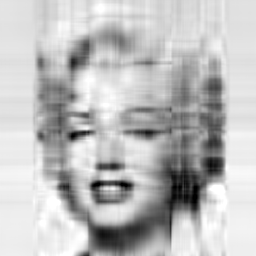
\includegraphics[width = 70mm]{k8.png}
\caption{mm.gif svd-dekomponert med $k=8$}
\end{center}
\end{figure}

og for $k = 32$:

\begin{figure}[H]
\begin{center}
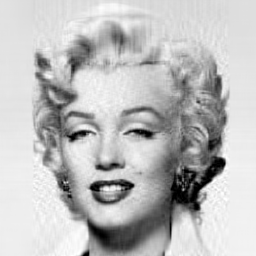
\includegraphics[width = 70mm]{k32.png}
\caption{mm.gif svd-dekomponert med $k=32$}
\end{center}
\end{figure}

Med $k = 8$ kan vi såvidt se at hvem bildet er av, og for $K=32$ er kan man helt tydelig se motivet. Man kan likevel se at bildet har blitt komprimert, særlig rundt halsen og håret. Vi burde med andre ord velge en noe større $k$ for at bildet skal ha en god kvalitet.

\subparagraph*{d)}

Figur 1 i oppgaveteksten består av nøyanser av sort til grå. Gjør vi dette til en matrise kan vil kolonnene bestå av de forskjellige "fargene". Alle elementene i en kolonne er like, hvilket betyr at radene i denne matrisen er like. Siden vi kan skrive rangen til denne matrisen som 

$$Rank(\bold{A}) = dim(Col(\bold{A})) = dim(Row(\bold{A}))$$

og alle radene er like, betyr det at dimensjonen på radrommet er 1, og derfor er rangen til dette bildet 1.

\subparagraph*{e)}

Jeg laget et lite progam jeg laget for å plotte $\sigma_j$

\lstinputlisting{plotSigma.m}


\end{document}
